\documentclass[letterpaper, 12pt]{math}

\usepackage{amsmath}
\usepackage{amssymb}
\usepackage{array}
\usepackage[linguistics]{forest}
\usepackage{pgfplots}

\pgfplotsset{compat=1.13}
\usepgfplotslibrary{fillbetween}
\usetikzlibrary{patterns}

\title{Probability and Statistics}
\author{Alvin Lin}
\date{Probability and Statistics: January 2017 - May 2017}

\begin{document}

\maketitle

\section*{Jointly Distributed Random Variables}
Let \( X \) and \( Y \) be two discrete random variables defined on the same
sample space \( S \) of an experiment. The joint pmf \( p(x,y) \) is defined
for any numbers \( x \) and \( y \) by:
\[ p(x,y) = P(X=x\ and\ Y=y) \]
The function \( p(x,y) \) satisfies the following properties.
\begin{enumerate}
  \item \( p(x,y) \geq 0 \) for any \( x,y \) \\
  \item \( \sum_{x}\sum_{y}p(x,y) = 1 \) \\
\end{enumerate}

\subsection*{Marginal PMF}
Marginal pmf of \( X \):
\[ p_{X}(x) = \sum_{y:p(x,y)>0}p(x,y) \]

\subsection*{Jointly Distributed Continuous Random Variables}
Let \( X \) and \( Y \) be continuous random variables. A joint pdf \( f(x,y) \)
satisfies the following conditions.
\begin{enumerate}
  \item \( P((X,Y)\in A) = \int_{A}\int f(x,y)\diff{x}\diff{y} \)
  \item \( f(x,y)\geq 0\ for\ any\ x\ and\ y \) \\
  \item \( \int_{-\infty}^{\infty}\int_{-\infty}^{\infty}
    f(x,y)\diff{x}\diff{y} = 1 \)
\end{enumerate}

\subsection*{Example}
A hat contains two balls marked 1 and one ball marked 2. Select a ball randomly,
and then with replacement select a ball randomly. Let \( X \) be the number on
the first ball and \( Y \) be the number on the second ball. Let \( p(x,y) \)
be the joint pmf of \( X \) and \( Y \). Let \( p(x) \) and \( p(y) \) be the
marginal pmf of \( X \) and \( Y \) respectively.
\begin{center}
  \begin{forest}
    [
      [1 [1] [1] [2] ]
      [1 [1] [1] [2] ]
      [2 [1] [1] [2] ]
    ]
  \end{forest}
\end{center}
\begin{equation*}
  \begin{aligned}[c]
    p_{x}(1) &= \sum_{y}p(1,y) \\
    &= p(1,1)+p(1,2) \\
    &= \frac{4}{9}+\frac{2}{9} = \frac{6}{9} \\
    p_{x}(2) &= \sum_{y}p(2,y) \\
    &= p(2,1)+p(2,2) \\
    &= \frac{2}{9}+\frac{1}{9} = \frac{3}{9} \\
  \end{aligned}
  \quad\quad
  \begin{aligned}[c]
    p_{y}(1) &= \sum_{x}p(x,1) \\
    &= p(1,1)+p(2,1) \\
    &= \frac{4}{9}+\frac{2}{9} = \frac{6}{9} \\
    p_{y}(2) &= \sum_{x}p(x,2) \\
    &= p(1,2)+p(2,2) \\
    &= \frac{2}{9}+\frac{1}{9} = \frac{3}{9}
  \end{aligned}
\end{equation*}
\begin{center}
  {\renewcommand{\arraystretch}{2}
  \begin{tabular}{|c|c|c|c|c|c|}
    \hline
    \( x \) & \( y \) & \( p_{x}(x) \) & \( p_{y}(y) \) &
      \( p_{x}(x)\cdot p_{y}(y) \) & \( p(x,y) \) \\
    \hline
    1 & 1 & \( \frac{6}{9} \) & \( \frac{6}{9} \) &
      \( \frac{36}{81} = \frac{4}{9} \) & \( \frac{4}{9} \) \\
    \hline
    1 & 2 & \( \frac{6}{9} \) & \( \frac{3}{9} \) &
      \( \frac{18}{81} = \frac{2}{9} \) & \( \frac{2}{9} \) \\
    \hline
    2 & 1 & \( \frac{3}{9} \) & \( \frac{6}{9} \) &
      \( \frac{18}{81} = \frac{2}{9} \) & \( \frac{2}{9} \) \\
    \hline
    2 & 2 & \( \frac{3}{9} \) & \( \frac{3}{9} \) &
      \( \frac{9}{81} = \frac{1}{9} \) & \( \frac{1}{9} \) \\
    \hline
  \end{tabular}}
\end{center}
\[ p_{x}(1) = P(X=1) = \frac{6}{9} \]
\( X \) and \( Y \) are independent. Find the conditional probability function
of \( Y \) given that \( X = 2 \).
\[ p_{y|x}(y|2) = \frac{p(2,y)}{p_{x}(2)} = \begin{cases}
  \frac{3}{3} &, y = 1 \\
  \frac{1}{3} &, y = 2 \\
  0 &, otherwise\end{cases}
\]
Suppose we have \( p_{y|x}(1|2) \). This represents the probability that
\( Y = 1 \) given \( X = 2 \). Of the sample space, the new subspace consists
of:
\begin{center}
  \begin{forest}
    [
      2 [1] [1] [2]
    ]
  \end{forest}
\end{center}
\[ p_{y|x}(1|2) = P(Y=1\ given\ that\ X=2) = \frac{2}{3} \]

\subsection*{Double Integral}
If \( f(x)\geq0 \) for any \( x\in\R \), \( \int_{1}^{3}f(x)\diff{x} \) is
the area under the curve \( y = f(x) \), \( x\in[1,3] \). If \( f(x,y)\geq0 \)
for any \( (x,y)\in\R^{2} \), \( \int_{1}^{2}\int_{1}^{3}f(x,y)\diff{x}\diff{y}
\) is the volume under the surface \( \delta = f(x,y) \) where:
\[ (x,y)\in A = \{(x,y)\in\R^{2}\mid 1\leq x\leq 3\ and\ 1\leq y\leq 2 \} \]
Suppose \( f(x,y) \) is the joint pdf uniformly distributed on the rectangle
\( A \), then:
\[ f(x,y) = \begin{cases}
  c &, (x,y)\in A \\
  0 &, otherwise\end{cases}
\]
How do we find the value of the constant \( c \)?
\begin{equation*}
  \begin{aligned}[t]
    1 &= \int_{-\infty}^{\infty}\int_{-\infty}^{\infty}f(x,y)\diff{x}\diff{y} \\
    &= \int\int_{A}f(x,y)\diff{x}\diff{y} \\
    &= \int\int_{A}c\diff{x}\diff{y} \\
    &= c\int\int_{A}\diff{x}\diff{y} \\
    &= c\bigg[area\ of\ A\bigg] \\
    &= c(2-1)(3-1) \\
    c &= \frac{1}{2}
  \end{aligned}
  \quad\quad
  \begin{aligned}[t]
    1 &= \int_{-\infty}^{\infty}\int_{-\infty}^{\infty}f(x,y)\diff{x}\diff{y} \\
    &= \int\int_{A}f(x,y)\diff{x}\diff{y} \\
    &= \int\int_{A}c\diff{x}\diff{y} \\
    &= c\int\int_{A}\diff{x}\diff{y} \\
    &= c\int_{1}^{2}\bigg[\int_{1}^{3}\diff{x}\bigg]\diff{y} \\
    &= c\int_{1}^{2}\bigg[x\bigg]_{x=1}^{x=3}\diff{y} \\
    &= c\int_{1}^{2}\bigg[3-1\bigg]\diff{y} \\
    &= c(3-1)\int_{1}^{2}\diff{y} \\
    &= c(3-1)\bigg[y\bigg]_{y=1}^{y=2} \\
    &= c(3-1)(2-1) \\
    c &= \frac{1}{2}
  \end{aligned}
\end{equation*}
The volume under the curve is numerically equal to the area of \( A \) even
though they are dimensionally different because the surface is flat and its
height is equal to 1.

\subsection*{Example}
Annie and Alvie have agreed to meet between 5:30PM and 6:00PM for dinner
at a local health-food restaurant. Let \( X = Annie's\ arrival time \) and
\( Y = Alvie's\ arrival\ time \). Suppose \( X \) and \( Y \) are independent
with each uniformly distributed on the interval [5:30,6:00]
( \( [5.5,6] \) ). What is the joint pdf of \( X \) and \( Y \)? \par
Let \( A = \{(x,y)\in\R^{2}\mid 5.5\leq x\leq 6\and 5.5\leq y\leq 6\} \).
\[ f(x,y) = \begin{cases}
  c &, (x,y)\in A \\
  0 &, otherwise\end{cases}
\]
\begin{align*}
  1 &= \int_{-\infty}{\infty}\int_{-\infty}{\infty}f(x,y)\diff{x}\diff{y} \\
  &= \int\int_{A}f(x,y)\diff{x}\diff{y} \\
  &= \int\int_{A}c\diff{x}\diff{y} \\
  &= c\bigg[area\ of\ A\bigg] \\
  &= c\cdot\frac{1}{2}\cdot\frac{1}{2} \\
  c &= 4 \\
  f(x,y) &= \begin{cases}
    4 &, (x,y)\in A \\
    0 &, otherwise
  \end{cases}
\end{align*}
What is the probability that both arrive between 5:15 and 5:45? \par
The area of overlap is only between 5:30 and 5:45, so the area is
\( \frac{1}{4}\cdot\frac{1}{4} \).
\[ \frac{overlap}{total} =
   \frac{\frac{1}{4}\cdot\frac{1}{4}}{\frac{1}{2}\cdot\frac{1}{2}} = \frac{1}{4}
\]
If the first one to arrive will wait only 10 minutes before leaving to eat
elsewhere, what is the probability that Annie arrives before Alvie and that
they have dinner at the health-food restaurant? We can write these conditions
as follows:
\[ |x-y|\leq\frac{1}{6} \]
\[ x\leq y \]
\[ -\frac{1}{6}\leq x-y\leq\frac{1}{6} \]
\[ y\leq x+\frac{1}{6} \]
\[ x-\frac{1}{6}\leq y \]
\[ y\geq x-\frac{1}{6} \]
\begin{center}
  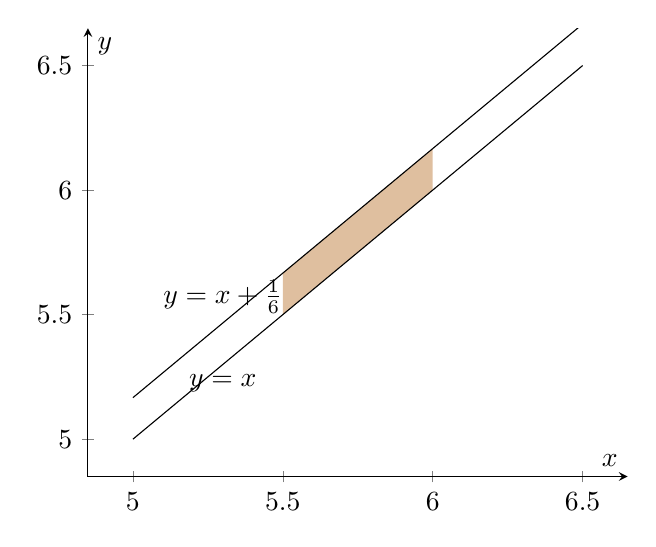
\begin{tikzpicture}
    \begin{axis}[axis lines=middle,
                 xlabel=\(x\),
                 ylabel=\(y\),
                 enlargelimits,
                 xmin=5, xmax=6.5,
                 ymin=5, ymax=6.5
                ]
    \addplot[name path=F, black, domain={5:6.5}]{x}
        node[pos=0.2, below]{\( y=x \)};
    \addplot[name path=G, black, domain={5:6.5}]{x+(1/6)}
        node[pos=0.2, above]{\( y=x+\frac{1}{6} \)};
    \addplot[color=brown!50] fill between [
             of=F and G, soft clip={domain=5.5:6}];
    \end{axis}
  \end{tikzpicture}
\end{center}
The area of this region (trapezoidal) is:
\[ \frac{1}{2}\cdot\frac{1}{2}\cdot\frac{1}{2}-\frac{1}{2}(\frac{1}{2}-
   \frac{1}{6})^{2} = \frac{1}{8}-\frac{1}{18} \]
\[ P = \frac{area}{total} =
   \frac{\frac{1}{8}-\frac{1}{18}}{\frac{1}{2}\cdot\frac{1}{2}} \]

\begin{center}
  If you have any questions, comments, or concerns, please contact me at
  alvin@omgimanerd.tech
\end{center}

\end{document}
